\subsection{Optimizing layer combination}

In this subsection we describe the methods to answer the following research questions:
\begin{itemize}
    \item \textbf{RQ3}: How does adding ALC and BLC to LightGCN perform compared to other state of the art methods?
    \item \textbf{RQ4}: Is it beneficial to change layer combination based on the degree of the nodes?
\end{itemize}  

\subsubsection{Degree based layer combination}
\todo{Omskriv denne til at passe med rød tråd og passe bedre med det vi har lavet}
\todo{consider if RQ4 should be two different and more specific research questions}
The initial idea of optimizing $\alpha_k$ was to change each layer's effect depending on how many connections each node had.
An example can be seen \autoref{tab:alpha-example}.
The numbers shown on the table are arbitrary and different variables need to be tested to see how well it performs.
The intuition behind this is that the effect of each layer in the GCN being dependent on the number of connections that the node has would be beneficial.
A node with only 1 connection will not benefit much from the first convolution but will be richer in information in the third convolution.
For a node with 200 connections, the third convolution might actually be harmful, as the node gets impacted too much by too many nodes, where 1 convolution is enough to make it perform optimally.

\begin{table}[]
    \centering
    \begin{tabular}{|l|l|}
        \hline
        Number of connections & Effect of each layer      \\ \hline
        0 - 20                & \begin{tabular}[c]{@{}l@{}}10 \% effect of $e^{(0)}$\\ 15 \% effect of $e^{(1)}$\\ 25 \% effect of $e^{(2)}$\\ 50 \% effect of $e^{(3)}$\end{tabular} \\ \hline
        21-50                 & \begin{tabular}[c]{@{}l@{}}10 \% effect of $e^{(0)}$\\ 10 \% effect of $e^{(1)}$\\ 60 \% effect of $e^{(2)}$\\ 20 \% effect of $e^{(3)}$\end{tabular} \\ \hline
        50+                   & \begin{tabular}[c]{@{}l@{}}10 \% effect of $e^{(0)}$ \\ 50 \% effect of $e^{(1)}$\\ 20 \% effect of $e^{(2)}$ \\ 20 \% effect of $e^{(3)}$\end{tabular} \\ \hline
    \end{tabular}
    \caption{Example of the changed effect to $\alpha_k$. }
    \label{tab:alpha-example}
\end{table}

\paragraph{Layer effect based on performance} \label{fredsplit}
\todo{Omskriv således at det introducere ALC / BLC i hver sin og som fokuserer på forskellen mellem dem}
%%% Måske sandt, men er ikke så god en intro når læseren ikke er kommet dertil.
% Based on the results from the node degree experiments seen in \autoref{subsec:degree-experiment}, we decided to make an algorithm that calculated each layers' effect based on how they performed compared to each other.
% It could clearly be seen that some layers performed substantially better than others and therefore the worst layers might have a negative effect on the final embedding.
Instead of utilizing average as the weighted sum, two algorithms were developed to do weighted sum based on the performance of each layer.
The algorithm looks at the performance of each individual layer and then based on how much worse they perform compared to the best layer they will get a penalty in their effect and the other layers will get an increase.
Two algorithms have been created where one has a more aggressive approach, that can completely remove certain layers, and the other one has a more balanced approach, where each layer will be ensured influence.
An advantage to the aggressive algorithm is that it is able to completely remove certain layers that has performed poorly, but there seems to be a beneficial factor to aggregating different layers, which in some cases will be eliminated with this algorithm.
For the balanced algorithm, it ensures that all layers will have influence, but in some cases an layer might perform so bad, that it is harmful to add it.
An example of the aggressive algorithm can be seen on \autoref{fig:fredsplitAgg} and an example of the balanced algorithm can be seen on \autoref{fig:fredsplitBal}.
Given four layers on \autoref{fig:fredsplitAgg} each layer will have 25\% effect on the final embedding initially.
The worst layer performs 15\% worse than the best layer, we therefore remove 15 from 25 to get its final effect of 10.
Meanwhile, the 15 is split evenly among the 3 other layers who now have an effect of 30\%.
The same process is then repeated but the worst performing layer from the previous iteration is excluded.
This continues until all layers have gotten an effect penalty except the best performing layer.
This can result in one or more layers having 0 \% effect in the end.
In the balanced version the worst-performing layer is not excluded from the previous iteration.
\\
On \autoref{alg:aggresive-layereffect} the pseudocode for the aggressive algorithm can be seen.
The algorithm is given a list of how much worse each layer performed in percentages compared to the best performing layer in the same list.
Initially each layers' \textit{effect} is set to be the same.
After this the list \textit{L} is iterated over and the last element gets popped.
Since L is ordered the last element is the worst performing one.
Based on the initial effect and the performance of the layer its effect is lowered while the other layers effect is increased.
On \autoref{alg:bal-layereffect} the pseudocode for the balanced method can be seen.
Examples of how the aggressive and balanced algorithms work can be seen on \autoref{fig:fredsplitAgg} and \autoref{fig:fredsplitBal}
In both examples we have 4 layers from 0 to 3 and each layer has an initial effect of 25\%.
Their performance is color coded to make it easier to follow which values are used to calculate the new effect.
The yellow squares mark which layer is getting a lower effect in the current iteration and green marks the specific layer's final effect.
Comparing these two algorithms it can be seen that there is a larger diversion in the aggressive algorithm than in the balanced algorithm.
\begin{algorithm}
    \caption{Algorithm for the aggressive layer combination based on performance}
    \SetAlgoLined
    \KwResult{A list of how much effect each layer has on the final embedding }
    L = Ordered list of performance of each layer \\
    effect  = List of current effect for each layer \\
    \While{i < L.length; i++}{
        effect [i] = 100 / L.length \\
    }
    \While{L.length > 1; i++}{
        worseP = L.pop()\\
        newEffect  = max(Inf[i] - worseP, 0)\\
        \While{k < L.length; k++}{
            effect[k] = effect[k] + ((effect[i] - newEffect ) / L.length)\\
        }
        effect[i] = newEffect \\
    }
    \Return{effect.orderBy(layerId)}
    \label{alg:aggresive-layereffect}
\end{algorithm}

\begin{algorithm}
    \caption{Algorithm for the balanced layer combination based on performance}
    \SetAlgoLined
    \KwResult{A list of how much effect each layer has on the final embedding }
    L = Ordered list of performance of each layer \\
    effect  = List of current effect for each layer \\
    \While{i < L.length; i++}{
        effect [i] = 100 / L.length \\
    }
    \While{i = 0; i < L.length; i++}{
        worseP = L.[i]\\
        newEffect  = max(effect[i] - worseP, 0)\\
        \While{k = 0; k < L.length; k++}{
            if(k != i){
                    effect[k] = effect[k] + ((effect[i] - newEffect ) / (L.length-1))\\
                }
        }
        effect[i] = newEffect \\
    }
    \Return{effect.orderBy(layerId)}
    \label{alg:bal-layereffect}
\end{algorithm}


\begin{figure}
    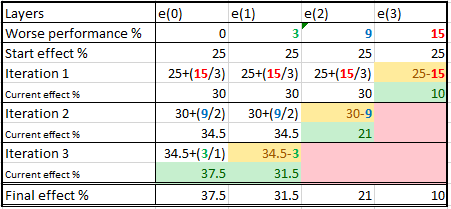
\includegraphics[width=0.5\textwidth]{figures/fredsplit/aggresiveAlgo.png}
    \centering
    \caption{Example of aggressive splitting of layer effect based on performance}
    \label{fig:fredsplitAgg}
\end{figure}

\begin{figure}
    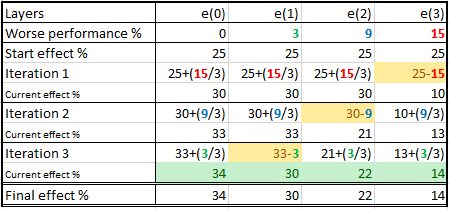
\includegraphics[width=0.5\textwidth]{figures/fredsplit/balancedAlgo.png}
    \centering
    \caption{Example of balanced splitting of layer effect based on performance}
    \label{fig:fredsplitBal}
\end{figure}
